\documentclass[14pt]{extarticle}
\usepackage{amsmath}
\usepackage{amssymb}
\usepackage{tikz}
%\usetikzlibrary{calc}
\usetikzlibrary{trees}
\usepackage{hyperref}
\usepackage{graphicx}
\graphicspath{ {../../chap08/} }
\usepackage[top=0.75in, bottom=0.75in, left=0.75in, right=0.75in]{geometry}
\newcommand*{\Scale}[2][4]{\scalebox{#1}{\ensuremath{#2}}}%
\usepackage[shortlabels]{enumitem}
\usepackage[most]{tcolorbox}
\definecolor{bg}{RGB}{255,249,227}
% \usepackage{showframe}
\title{\vspace{-5ex}Math 208 Section 8.3}
\date{\vspace{-10ex}}
\usepackage{multicol}
\setlength{\columnsep}{1cm}


\begin{document}
\maketitle		
\section*{Homework, Reading, and Other}
\begin{itemize}
	\item Section 7.3, 7.4
	\item Section 8.1, 8.2
	\item Section 8.3
\end{itemize}

\section{Goals}
\begin{itemize}
	\item Understand, apply, and analyze conditional probability
	\item Utilize a Probability Tree
	\item Understand, apply, and analyze Independence and its relation to conditional probability
\end{itemize}

\section{8.3: Conditional Probability, Intersection, and Independence}
Conditional Probability is how we update our thinking of event likelihood based upon new information.
\\\\
For example, what is the probability that a person has received the Covid vaccine? Less than 30\% right?
\\\\
If I told you the person was in their 80s, would you like to change your guess?


\subsection{Conditional Probability}
That is \textbf{conditional probability}, $P(A|B)$, the probability that A occurs given B has occurred. Here are some other examples:
\begin{itemize}
	\item Probability of drawing a heart given the card is red
	\item Probability of lung cancer given the person smoked
\end{itemize}
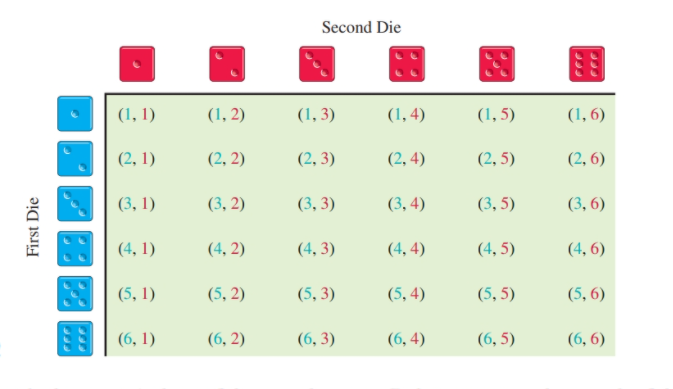
\includegraphics[width=0.9\linewidth]{8-1-5}
\\
Recalling the two-dice sample space in the table, consider the probability of rolling a 7 given the roll is odd. Lets count that, there are 18 odd events and 6 events that roll a 7. Let A is the event of rolling a 7 and B is the event of rolling an odd.
$$P(A|B) = \frac{6}{18}$$
Let's look at this more closely.
\begin{tcolorbox}[enhanced jigsaw,colback=bg,boxrule=0pt,arc=0pt] 
	\textbf{Conditional Probability}
	\begin{align*}
		P(A|B)&=\frac{n(A\cap B)}{n( B)} = \frac{\frac{n(A\cap B)}{n(S)}}{\frac{n(B)}{n(S)}} \\
		&= \frac{P(A\cap B)}{P(B)}
	\end{align*}
and
\begin{align*}
	P(B|A)&=\frac{n(A\cap B)}{n(A)} \\
	&= \frac{P(A\cap B)}{P(A)}
\end{align*}
You will often use both methods to find conditional probability
\end{tcolorbox}

\subsubsection{Examples}
\begin{enumerate}
	\item What is the probability that only one of the dice is a 2, event A, given the total is less than 7, event B?
	\begin{align*}
		n(S) &= 36 \\
		n(B) &= 15 \\
		n(A \cap B) &= 6 \\
		P(B) &= 15/36  \\
		P(A\cap B)&= 6/36 \\
		P(A|B) = \frac{P(A\cap B)}{P(B)} = \frac{6*36}{15*36} &= 6/15
	\end{align*}

	\item A pointer is spun once on a circular spinner. The probabilities of the pointer landing on a given integer from 1 to 6 are given in the table.
	\\
	\begin{tabular}{|c|c|c|c|c|c|r|}
		\hline
		Integer & 1 & 2 & 3 & 4 & 5 & 6 \\
		\hline
		P(Int) & .1 & .2 & .1 & .1 & .3 & .2 \\
		\hline
	\end{tabular}
	\begin{enumerate}
		\item What is the probability the pointer lands on a prime number?
		$$P(E) = P(\text{prime}) = P(2) +P(3)+P(5) = 0.6$$
		\item What is the probability of the pointer landing on a prime number, given that it landed on an odd number?
		\begin{align*}
			P(A) &= P(\text{odd})=P(1)+P(3)+P(5) = 0.5 \\
			P(E\cap A) &= P(3)+P(5) = 0.4 \\
			P(E|A) &= \frac{P(E\cap A)}{P(A)} = 0.4/0.5 = 0.8
		\end{align*}
	\end{enumerate}
\end{enumerate}

\subsection{Product Rule}
This is really just doing some algebra on the conditional probability equations. But it allows to find probabilities up and down the probability tree.

\begin{tcolorbox}[enhanced jigsaw,colback=bg,boxrule=0pt,arc=0pt] 
	\textbf{Product Rule}
	\begin{align*}
		P(A\cap B) = P(A)P(B|A) = P(B)P(A|B)
	\end{align*}
\end{tcolorbox}

\subsection{Probability Tree}
Probability trees are convenient tools for helping to compute probabilities of combined outcomes in a sequence of experiments. You've seen them before even though you might not have know waht they were called.

\subsubsection{Example 1}
Two balls are drawn in succession, without replacement, from a box containing 3 blue and 2 white balls. What is the probability of drawing a white ball on the second draw? Note that $S=\{WW, WB, BW, BB\}$.
\\\\

% Set the overall layout of the tree
\tikzstyle{level 1}=[level distance=4cm, sibling distance=4.0cm]
\tikzstyle{level 2}=[level distance=4cm, sibling distance=2cm]
% Define styles for bags and leafs
\tikzstyle{bag} = [text width=4em, text centered]
\tikzstyle{end} = [circle, minimum width=3pt,fill, inner sep=0pt]
\tikzset{
	treenode/.style = {shape=rectangle, rounded corners,
		draw, align=center,
		%top color=white, bottom color=blue!20
	},
	payoff/.style    = {align=center, inner sep=0.1em, text width=1.5em},
	left side node/.style={above left, inner sep=0.1em},
	right side node/.style={above right, inner sep=0.1em}
}

\begin{tikzpicture}
	[
	grow                    = right,
	sibling distance        = 10em,
	level distance          = 4em,
%	every node/.style       = {font=\footnotesize},
	sloped
	]
	\node [treenode] {Start}
		child{node [treenode] {B} 
		child{
			node [treenode] {B $\to \frac{3}{10}$} edge from parent node[left side node] {$2/4$}
		}
		child{
			node [treenode] {W $\to \frac{3}{10}$} edge from parent node[left side node] {$2/4$}
		}
		edge from parent node[right side node] {$3/5$}
	}
	child{node [treenode] {W} 
		child{
			node [treenode] {B $\to \frac{3}{10}$} edge from parent node[left side node] {$3/4$}
		}
		child{
			node [treenode] {W $\to \frac{1}{10}$} edge from parent node[left side node] {$1/4$}
		}
		edge from parent node[right side node] {$2/5$}
	};
\end{tikzpicture}
\\\\
The probabilities at the final leaves of the tree are intersection probabilities and are calculated by multiplying together each branch leading to it.
\begin{align*}
	\text{First Roll}&  \\
	&P(W) = 2/5, & P(B)=3/5 \\
	\text{Second Roll}&  \\
	&P(W|W) = 1/4, & P(B|W)=3/4 \\
	&P(W|B) = 2/4, & P(B|B)=2/4
\end{align*}
Then the probability of the intersection event is:
\begin{align*}
	&P(W\cap W) = 2/5 * 1/4 = 2/20 = 1/10 \\
	&P(W\cap B) = 2/5 * 3/4 = 6/20 = 3/10 \\
	&P(B\cap W) = 3/5 * 2/4 = 6/20 = 3/10 \\
	&P(B\cap B) = 3/5 * 2/4 = 6/20 = 3/10
\end{align*}
As a check on calculations, the sum of the leaves probabilities should equal 1. Sum(P)$=10/10=1$.
\\\\
Recall, we are asked what is $P(W$ on the second draw)? Sum up the probabilities that have W on the second draw. $P(*W) = P(W\cap W) + P(B\cap W) = 4/10$.

\begin{tcolorbox}[enhanced jigsaw,colback=bg,boxrule=0pt,arc=0pt] 
	\textbf{Draw a Probability Tree}
	\begin{enumerate}
		\item Draw a tree diagram corresponding to all combined outcomes of the sequence of experiments.
		\item Label each node.
		\item Assign a probability to each tree branch.
		\item Calculate intersection probabilities for the leaves or as needed.
		\item Answer questions related to the experiment
	\end{enumerate}
\end{tcolorbox}

\subsubsection{Example 2}
Rerun the experiment drawing balls experiment, only now replace any balls selected. Draw and then compare the probability trees.
\\\\
\begin{tikzpicture}
	[
	grow                    = right,
	sibling distance        = 10em,
	level distance          = 4em,
	%	every node/.style       = {font=\footnotesize},
	sloped
	]
	\node [treenode] {Start}
	child{node [treenode] {B} 
		child{
			node [treenode] {B $\to \frac{9}{25}$} edge from parent node[left side node] {$3/5$}
		}
		child{
			node [treenode] {W $\to \frac{6}{25}$} edge from parent node[left side node] {$2/5$}
		}
		edge from parent node[right side node] {$3/5$}
	}
	child{node [treenode] {W} 
		child{
			node [treenode] {B $\to \frac{6}{25}$} edge from parent node[left side node] {$3/5$}
		}
		child{
			node [treenode] {W $\to \frac{4}{25}$} edge from parent node[left side node] {$2/5$}
		}
		edge from parent node[right side node] {$2/5$}
	};
\end{tikzpicture}
\\\\
As a check on calculations, the sum of the leaves probabilities should equal 1. Sum(P)$=25/25=1$.
\\\\
This result is quite different than the previous result. With replacement lead to "independent" events while without replacement causes the result of subsequent draws to be "dependent".

\subsection{Independent Events}
For the independent events, we note that $P(A|B)=P(A)$, while for dependent events, this is not true. This allows us to develop a test for independence.
\begin{tcolorbox}[enhanced jigsaw,colback=bg,boxrule=0pt,arc=0pt] 
	\textbf{Independent Events}\\\\
	If A and B are any events in a sample space S, we say that A and B are \textbf{independent} if 
	$$ P(A\cap B) = P(A)P(B)$$
	Otherwise, A and B are said to be \textbf{dependent}.
	\\\\
	and \\\\
	If A and B are independent events with nonzero probabilities, then 
	\begin{align*}
		P(A|B) = P(A) & & P(B|A)=P(B)
	\end{align*}
\end{tcolorbox}

\subsubsection{Example}
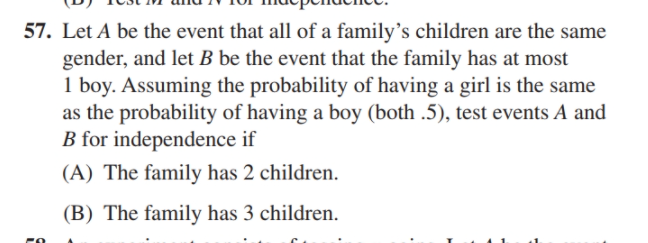
\includegraphics[width=0.9\linewidth]{8-3-6}
\\
What is the sample space?
\begin{align*}
	&S_2=\{GG, GB, BG, BB\} \\
	&S_3=\{GGG, GGB, GBG, GBB,BGG,BGB,BBG,BBB \}
\end{align*}
\\\\
Let's draw the tree.
\\\\
\tikzstyle{level 1}=[level distance=4cm, sibling distance=6.0cm]
\tikzstyle{level 2}=[level distance=4cm, sibling distance=3cm]
\tikzstyle{level 3}=[level distance=4cm, sibling distance=1.5cm]
\begin{tikzpicture}
	[
	grow                    = right,
	sibling distance        = 10em,
	level distance          = 4em,
	%	every node/.style       = {font=\footnotesize},
	sloped
	]
	\node [treenode] {Start}
	child{node [treenode] {B} 
		child{
			node [treenode] {B $\to \frac{1}{4}$}
			child{
				node [treenode] {B $\to \frac{1}{8}$} edge from parent node[left side node] {$1/2$}
			}
			child{
				node [treenode] {G $\to \frac{1}{8}$} edge from parent node[left side node] {$1/2$}
			}
			edge from parent node[left side node] {$1/2$}
		}
		child{
			node [treenode] {G $\to \frac{1}{4}$}
			child{
				node [treenode] {B $\to \frac{1}{8}$} edge from parent node[left side node] {$1/2$}
			}
			child{
				node [treenode] {G $\to \frac{1}{8}$} edge from parent node[left side node] {$1/2$}
			}
			edge from parent node[left side node] {$1/2$}
		}
		edge from parent node[right side node] {$1/2$}
	}
	child{node [treenode] {G} 
		child{
			node [treenode] {B $\to \frac{1}{4}$}
			child{
				node [treenode] {B $\to \frac{1}{8}$} edge from parent node[left side node] {$1/2$}
			}
			child{
				node [treenode] {G $\to \frac{1}{8}$} edge from parent node[left side node] {$1/2$}
			}
			edge from parent node[left side node] {$1/2$}
		}
		child{
			node [treenode] {G $\to \frac{1}{4}$}
			child{
				node [treenode] {B $\to \frac{1}{8}$} edge from parent node[left side node] {$1/2$}
			}
			child{
				node [treenode] {G $\to \frac{1}{8}$} edge from parent node[left side node] {$1/2$}
			}
			edge from parent node[left side node] {$1/2$}
		}
		edge from parent node[right side node] {$1/2$}
	};
\end{tikzpicture}
\\\\
\begin{itemize}
	\item Given 2 children, $A=\{GG, BB\}$ and $P(A)=1/4 + 1/4 = 1/2$
	\item Given 3 children, $A=\{GGG, BBB\}$ and $P(A)=1/8 + 1/8 = 1/4$
	\item Given 2 children, $B=\{GG, GB, BG\}$ and $P(B)=1/4 + 1/4 + 1/4= 3/4$
	\item Given 3 children, $B=\{GGG,GGB,GBG,BGG\}$ and $P(B)=4(1/8) = 1/2$
\end{itemize}
Are events A and B independent?
\begin{itemize}
	\item Given 2 children, $A\cap B = \{GGG\}$ and $P(A\cap B)= 1/4$. But $P(A)P(B)= (1/2)(3/4)=3/8$.
	\\\\
	A and B are dependent since $P(A\cap B) \neq P(A)P(B)$.$\blacksquare$
	\item Given 3 children, $A\cap B = \{GGG\}$ and $P(A\cap B)= 1/8$. But $P(A)P(B)= (1/4)(1/2)=1/8$.
	\\\\
	A and B are independent since $P(A\cap B) = P(A)P(B)$.$\blacksquare$
\end{itemize}


\noindent\rule{\textwidth}{1pt}
{\footnotesize Copyright (C) 2021 Garold Dalton --- Released under GNU General Public License v3.0}


\cleardoublepage


\end{document}
